% TODO:














%%%%%%%%%%%%%%%%%%%%%%%%%%%%%%%%%%%%%%%%%
% Beamer Presentation
% LaTeX Template
% Version 1.0 (10/11/12)
%
% This template has been downloaded from:
% http://www.LaTeXTemplates.com
%
% License:
% CC BY-NC-SA 3.0 (http://creativecommons.org/licenses/by-nc-sa/3.0/)
%
%%%%%%%%%%%%%%%%%%%%%%%%%%%%%%%%%%%%%%%%%

%----------------------------------------------------------------------------------------
%	PACKAGES AND THEMES
%----------------------------------------------------------------------------------------

\documentclass{beamer}

\mode<presentation> {

% The Beamer class comes with a number of default slide themes
% which change the colors and layouts of slides. Below this is a list
% of all the themes, uncomment each in turn to see what they look like.

%\usetheme{default}
%\usetheme{AnnArbor}
%\usetheme{Antibes}
%\usetheme{Bergen}
%\usetheme{Berkeley}
%\usetheme{Berlin}
%\usetheme{Boadilla}
%\usetheme{CambridgeUS}
%\usetheme{Copenhagen}
%\usetheme{Darmstadt}
%\usetheme{Dresden}
%\usetheme{Frankfurt}
%\usetheme{Goettingen}
%\usetheme{Hannover}
%\usetheme{Ilmenau}
%\usetheme{JuanLesPins}
%\usetheme{Luebeck}
\usetheme{Madrid}
%\usetheme{Malmoe}
%\usetheme{Marburg}
%\usetheme{Montpellier}
%\usetheme{PaloAlto}
%\usetheme{Pittsburgh}
%\usetheme{Rochester}
%\usetheme{Singapore}
%\usetheme{Szeged}
%\usetheme{Warsaw}

% As well as themes, the Beamer class has a number of color themes
% for any slide theme. Uncomment each of these in turn to see how it
% changes the colors of your current slide theme.

%\usecolortheme{albatross}
%\usecolortheme{beaver}
%\usecolortheme{beetle}
%\usecolortheme{crane}
%\usecolortheme{dolphin}
%\usecolortheme{dove}
%\usecolortheme{fly}
%\usecolortheme{lily}
%\usecolortheme{orchid}
%\usecolortheme{rose}
%\usecolortheme{seagull}
%\usecolortheme{seahorse}
%\usecolortheme{whale}
%\usecolortheme{wolverine}

%\setbeamertemplate{footline} % To remove the footer line in all slides uncomment this line
%\setbeamertemplate{footline}[page number] % To replace the footer line in all slides with a simple slide count uncomment this line

%\setbeamertemplate{navigation symbols}{} % To remove the navigation symbols from the bottom of all slides uncomment this line
}

\usepackage[utf8]{inputenc}
\usepackage[russian]{babel}
\usepackage{cmap}

\usepackage[absolute,overlay]{textpos}
\usepackage{verbatim}
\usepackage{fancybox}
\usepackage{ulem}
\usepackage{tikz}
\usetikzlibrary{positioning}
\usepackage{scalefnt}
\usetikzlibrary{arrows,shapes,positioning,shadows,trees,calc,backgrounds,fit,positioning}

\usepackage{graphicx} % Allows including images
\usepackage{booktabs} % Allows the use of \toprule, \midrule and \bottomrule in tables
\usepackage{textcomp}
\usepackage{listings}
\usepackage{color}
\usepackage{xcolor}
\usepackage{changepage}

\definecolor{mygreen}{rgb}{0,0.6,0}
\definecolor{mygray}{rgb}{0.5,0.5,0.5}
\definecolor{mymauve}{rgb}{0.58,0,0.82}

\lstset{ %
  backgroundcolor=\color{white},   % choose the background color; you must add \usepackage{color} or \usepackage{xcolor}
  basicstyle=\footnotesize,        % the size of the fonts that are used for the code
  breakatwhitespace=false,         % sets if automatic breaks should only happen at whitespace
  breaklines=true,                 % sets automatic line breaking
  captionpos=b,                    % sets the caption-position to bottom
  commentstyle=\color{mygreen},    % comment style
  deletekeywords={...},            % if you want to delete keywords from the given language
  escapeinside={\%*}{*)},          % if you want to add LaTeX within your code
  extendedchars=true,              % lets you use non-ASCII characters; for 8-bits encodings only, does not work with UTF-8
  frame=single,                    % adds a frame around the code
  keepspaces=true,                 % keeps spaces in text, useful for keeping indentation of code (possibly needs columns=flexible)
  keywordstyle=\color{blue},       % keyword style
  language=Octave,                 % the language of the code
  morekeywords={*,...},            % if you want to add more keywords to the set
  numbers=left,                    % where to put the line-numbers; possible values are (none, left, right)
  numbersep=5pt,                   % how far the line-numbers are from the code
  numberstyle=\tiny\color{mygray}, % the style that is used for the line-numbers
  rulecolor=\color{black},         % if not set, the frame-color may be changed on line-breaks within not-black text (e.g. comments (green here))
  showspaces=false,                % show spaces everywhere adding particular underscores; it overrides 'showstringspaces'
  showstringspaces=false,          % underline spaces within strings only
  showtabs=true,                  % show tabs within strings adding particular underscores
  stepnumber=1,                    % the step between two line-numbers. If it's 1, each line will be numbered
  stringstyle=\color{mymauve},     % string literal style
  tabsize=4,                       % sets default tabsize to 2 spaces
  %title=\lstname                   % show the filename of files included with \lstinputlisting; also try caption instead of title
}

%----------------------------------------------------------------------------------------
%	TITLE PAGE
%----------------------------------------------------------------------------------------

\graphicspath{{./figures/}}

\title[Обработка и исполнение запросов: лекция 7]{Обработка и исполнение запросов в СУБД (Лекция 7) \\~\\ Колоночные СУБД: схемы для OLAP; выполнение соединений в колоночных СУБД; сравнение с классическими СУБД\\~\\ v6} % The short title appears at the bottom of every slide, the full title is only on the title page

\author{Георгий Чернышев} % Your name
\institute[ВШЭ] % Your institution as it will appear on the bottom of every slide, may be shorthand to save space
{
Высшая Школа Экономики \\ % Your institution for the title page
\medskip
\textit{chernishev@gmail.com} % Your email address
}
%\date{\today} % Date, can be changed to a custom date
\date{14 октября 2020 г.}

\begin{document}

\begin{frame}
\titlepage % Print the title page as the first slide
\end{frame}

\begin{comment}
\begin{frame}
\frametitle{Overview} % Table of contents slide, comment this block out to remove it
\tableofcontents % Throughout your presentation, if you choose to use \section{} and \subsection{} commands, these will automatically be printed on this slide as an overview of your presentation
\end{frame}
\end{comment}

\begin{frame}
\frametitle{Про OLAP ``на пальцах''}

%\begin{figure}[htb]
%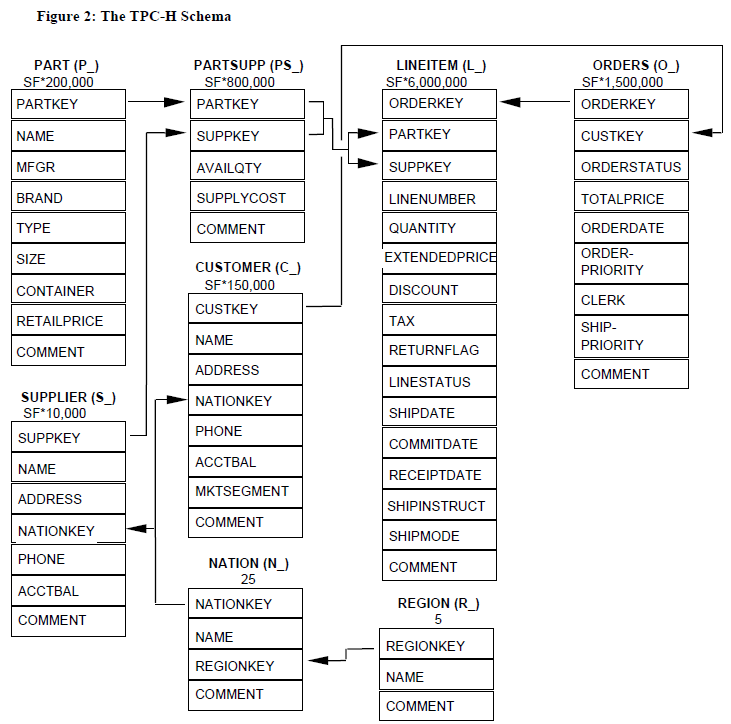
\includegraphics[width=\textwidth,height=0.50\textheight,keepaspectratio]{tpc-h.png} 
%\footnote{\tiny{Изображение взято из \cite{TPC-H}}}
% \end{figure}    

\begin{itemize}
  \setlength\itemsep{1em}
  \item OLAP базы данных имеют специальную схему: Star Schema, Snowflake Schema, ...
  \item Таблица фактов: хранит основные записи
  \begin{itemize}
    \item Большая, на несколько порядков больше таблиц измерений;
    \item Широкая, сотни атрибутов;
    \item Много FK, кроме них есть еще меры;
  \end{itemize}
  \item Таблицы измерений: 
  \begin{itemize}
    \item Количество записей мало, не широкие;
    \item Данные изменяются редко, в основном добавления;
  \end{itemize}
  
\end{itemize}

На самом деле всё сложнее, м.б. потом отдельно поразбираем OLAP.

\end{frame}

\begin{frame}
\frametitle{Схема ``звезда'', пример}

\begin{figure}[htb]
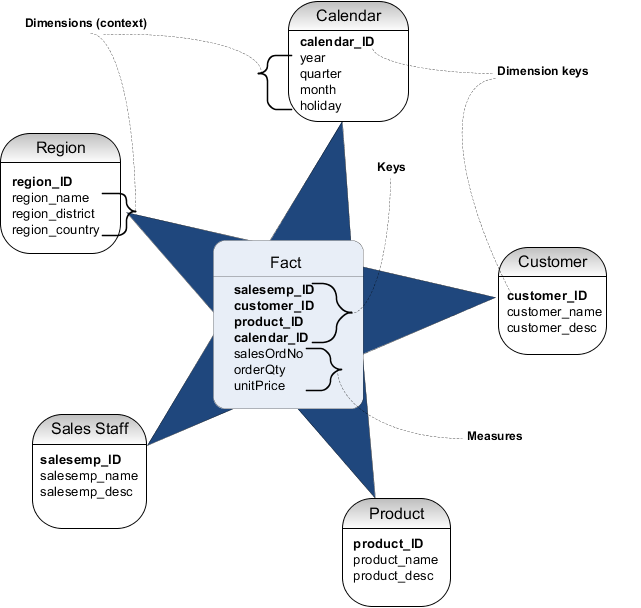
\includegraphics[width=\textwidth,height=0.750\textheight,keepaspectratio]{star-schema-1.png} 
\footnote{\tiny{Изображение взято из \url{https://docs.infor.com/help_lawson_cloudsuite_10.0/topic/com.lawson.help.reporting/com.lawson.help.bpwag-w_10.4.0/L55461185818015.html}}}
 \end{figure}    

\end{frame}

\begin{frame}
\frametitle{Схема ``снежинка'', пример}

\begin{figure}[htb]
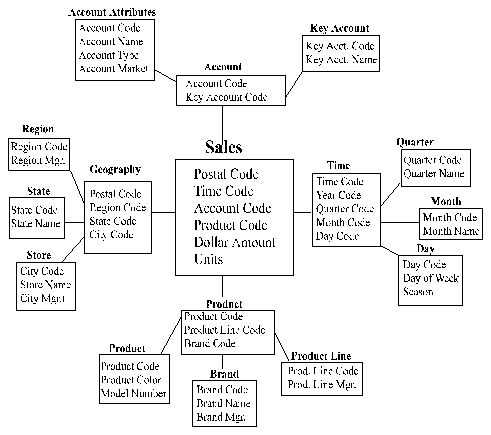
\includegraphics[width=\textwidth,height=0.750\textheight,keepaspectratio]{snowflake.png} 
\footnote{\tiny{Изображение взято из \url{http://www.informix.com.ua/articles/rolap/rolap.htm}}}
 \end{figure}    

\end{frame}


\begin{frame}
\frametitle{Итоги прошлой лекции}

\begin{figure}[htb]
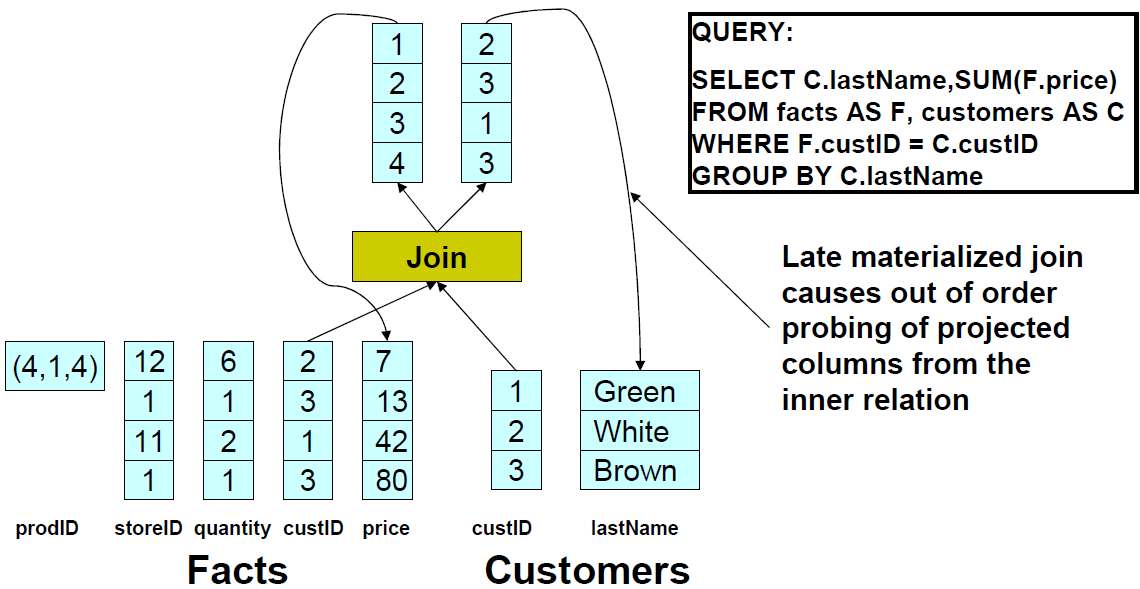
\includegraphics[width=\textwidth,height=0.50\textheight,keepaspectratio]{lm-join1.png} 
\footnote{\tiny{Изображение взято из \cite{Harizopoulos2009}}}
\end{figure}    

Соединения и поздняя материализация ``не дружат'':

\begin{itemize}
  \setlength\itemsep{1em}
  \item По одной из колонок теряется отсортированность;
  \item Вычитка несортированной колонки очень дорога;
\end{itemize}
$\longrightarrow$ нужны другие операторы соединения, специализированные для этих нагрузок

\end{frame}


\begin{frame}
\frametitle{Жесткий диск}

\begin{figure}[htb]
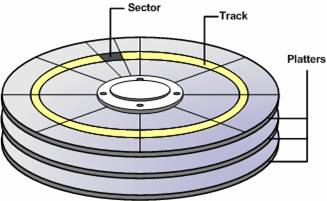
\includegraphics[width=\textwidth,height=0.320\textheight,keepaspectratio]{harddisk.png} 
\footnote{\tiny{Изображение взято из \url{http://www.applexsoft.com/glossary/hard-disk.html}}}
\end{figure}    
Затраты времени:
\begin{itemize}
  \item Seek time + Rotational latency = около 2.5 ms
  \item Command processing time = мало
  \item Settle time = мало
\end{itemize}
Считать с диска 100 элементов случайным доступом~--- 250ms. Последовательно: 2.5ms + 0.1ms.\\
$\longrightarrow$ надо избегать случайного доступа

\end{frame}

\begin{frame}
\frametitle{OLAP Benchmarks}

$\longrightarrow$ нужны эффективные операторы соединения\\~\\

Как? Использовать особенности OLAP, примеры:

\begin{itemize}
  \setlength\itemsep{1em}
  \item TPC-H \cite{TPC-H};
  \item Star Schema Benchmark \cite{SSB}~--- модицифированный TPC-H, исправляет недостатки TPC-H;
  \item Другие: TPC-DS.
\end{itemize}

\end{frame}



\begin{frame}
\frametitle{Star Schema Benchmark}

\begin{figure}[htb]
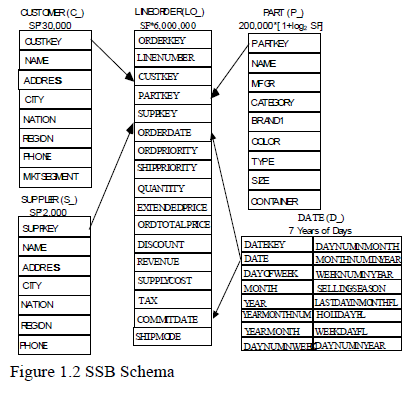
\includegraphics[width=\textwidth,height=0.750\textheight,keepaspectratio]{ssb.png} 
\footnote{\tiny{Изображение взято из \cite{SSB}}}
\end{figure}   

\end{frame}



% \cite{Abadi2008}


\begin{frame}[fragile]
\frametitle{Невидимое соединение}

\lstset{language=SQL}

\begin{lstlisting}
SELECT 
    c.nation, s.nation, d.year, sum(lo.revenue) as revenue
FROM customer AS c, lineorder AS lo,
    supplier AS s, dwdate AS d
WHERE lo.custkey = c.custkey
    AND lo.suppkey = s.suppkey
    AND lo.orderdate = d.datekey
    AND c.region = 'ASIA'
    AND s.region = 'ASIA'
    AND d.year >= 1992 and d.year <= 1997
GROUP BY c.nation, s.nation, d.year
ORDER BY d.year asc, revenue desc;
\end{lstlisting}

\end{frame}

\begin{frame}
\frametitle{Как вычислять запрос?}

Стратегии:

\begin{itemize}
  \setlength\itemsep{1em}
  \item Классический подход (ранняя материализация):
  \begin{itemize}
    \item Предикаты спустить вниз на уровень измерений;
    \item Упорядочить соединения по убыванию селективности;
    \item Результат сгруппировать и посчитать агрегатные функции;
  \end{itemize}
  \item Поздняя материализация:
  \begin{itemize}
    \item Применяем c.region = 'ASIA', получаем ключи у Customer;
    \item Соединяем с Fact Table, получаем позиции для LineOrder и Customer;
    \item Кто-то из них будет не отсортирован (обычно dimension) :(
    \item Забираем из customer атрибут c.nation по позициям (не отсортированы) и отсортированные данные из LineOrder (supplier key, order date, revenue);
    \item Аналогично соединяем supplier и date;
  \end{itemize}
\end{itemize}

\end{frame}

\begin{frame}
\frametitle{Как вычислять запрос? II}

Оба подхода плохи:

\begin{itemize}
	\setlength\itemsep{1em}
	\item Классический подход (ранняя материализация). Нет выигрышей от поздней материализации:
	\begin{itemize}
		\item нельзя поэкономить на чтении с диска;
		\item нет улучшения локальности кешей;
		\item нет возможности оперировать над сжатыми данными.
	\end{itemize}
	\item Поздняя материализация:
	\begin{itemize}
		\item Значения в dimensions не отсортированы, придется вытаскивать их не по порядку. Что весьма дорого.
	\end{itemize}
\end{itemize}

Выход~--- оператор Invisible Join: поздняя материализация и минимизация количества значений читаемых не по порядку.

\end{frame}

\begin{frame}
\frametitle{Invisible Join I}

Идея: переписать соединения в предикаты на FK колонки в таблице фактов. Шаги алгоритма:
\begin{enumerate}
  \item Применяем предикаты к таблицам измерений, получаем ключи;
  \item На ключах строится хеш-таблица (т.е. будем проверять правда ли что строка с данным значением ключа удовлетворяет предикату);
\end{enumerate}

\begin{figure}[htb]
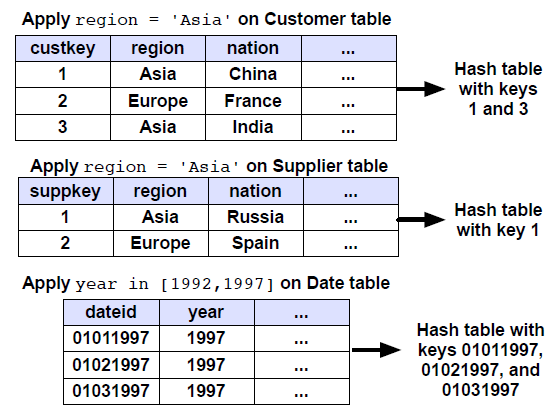
\includegraphics[width=\textwidth,height=0.50\textheight,keepaspectratio]{i1.png} 
\footnote{\tiny{Изображение взято из \cite{Abadi2008}}}
\end{figure}   

\end{frame}


\begin{frame}
\frametitle{Invisible Join II}

\begin{enumerate}
  \setcounter{enumi}{2}
  \item Идем по таблице фактов, опрашивая хеш-таблицы, от каждой получаем список позиций (записи удовлетворяющие предикату);
  \item Полученные списки позиций пересекаем;
\end{enumerate}

\begin{figure}[htb]
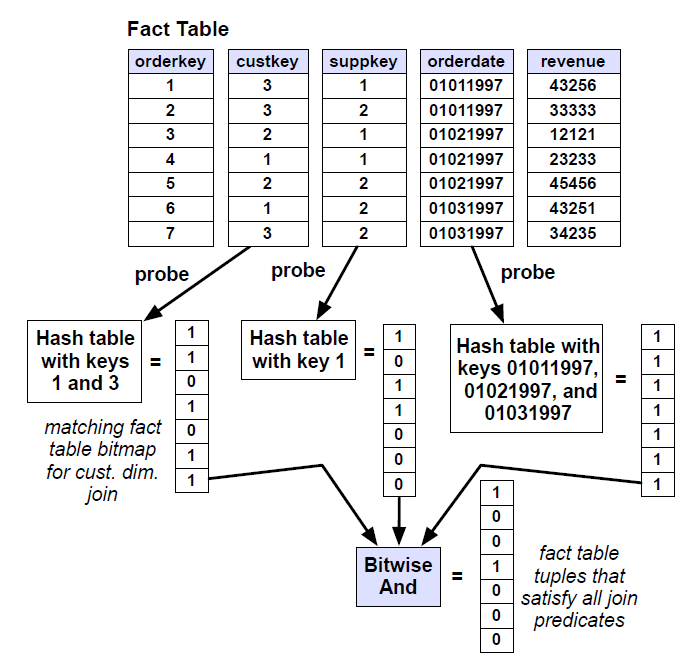
\includegraphics[width=\textwidth,height=0.650\textheight,keepaspectratio]{i2.png} 
\footnote{\tiny{Изображение взято из \cite{Abadi2008}}}
\end{figure}   

\end{frame}

\begin{frame}
\frametitle{Invisible Join III (схема)}

\begin{figure}[htb]
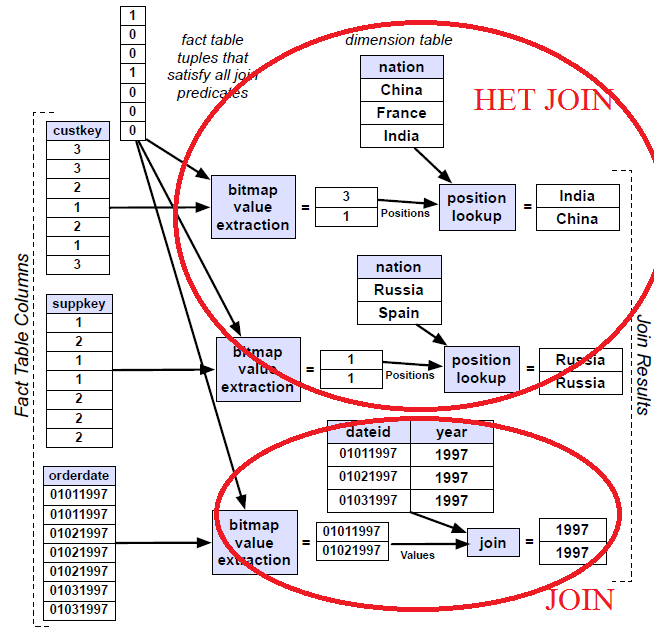
\includegraphics[width=\textwidth,height=0.800\textheight,keepaspectratio]{i3.png} 
\footnote{\tiny{Изображение взято из \cite{Abadi2008}}}
\end{figure}   

\end{frame}

\begin{frame}
\frametitle{Invisible Join III (описание)}

\begin{enumerate}
  \setcounter{enumi}{4}
  \item Из таблицы фактов получаем позиции в измерениях;
  \item Идем в таблицы измерений и забираем значения;
  \begin{enumerate}
    \item Если ключи в измерении отсортированы и начинаются с 1 то можно делать position lookup, фактически как массиве;
    \item Колонка в таблицах измерений обычно маленькая, помещается в L2 кеш, поэтому всё быстро;  
    \item Если ключи не отсортированы и не плотны, то придется соединять (последний случай на схеме в предыдщуем слайде);
    \item Соединять не так плохо как кажется: будет только один результат в каждой таблице измерений, значит будет одинаковое количество результатов в каждой таблице измерений, значит соединения можно параллелить и комбинировать результат после!
    \item Высокая селективность помогает выбирать меньше на этом шаге;
  \end{enumerate}  
\end{enumerate}

Оставляем таблицу фактов отсортированной всегда!

\end{frame}

\begin{comment}

\begin{frame}
\frametitle{Between predicate rewrite}

Если в таблице измерений ключи последовательны и без ``дыр'', а также предикату удовлетворет большая группа последовательных значений, например $[1000;2000]$,
тогда можно заменить хеш-таблицу на предикат between.

\begin{itemize}
  \item При соединении просто проверяем, правда ли что FK лежит в границах!
\end{itemize}

Требования довольно часто удовлетворены: колонки отсортированы по иерархиям, плюс roll-up запросы.

\end{frame}

\end{comment}

\begin{frame}
\frametitle{Jive join: описание}

Алгоритм соединения с использованием Join Index. Делаем интервальное фрагментирование, затем каждый фрагмент обрабатываем.\\~\\

Делает один \underline{последовательный} проход по каждому из отношений и два \underline{последовательных} просмотра временного файла. При этом, размер вспомогательного файла составляет половину от размера Join Index.\\~\\

Алгоритм требует наличия свободной памяти (блоков) порядка квадратного корня из размера (в блоках) из наименьшего отношения.\\~\\

Join Index: вспомогательная структура данных, позволяющая ускорить соединение. Устройство: список пар (id записи в первой таблице, id записи во второй).

\end{frame}

\begin{frame}
\frametitle{Jive join I}

Старый метод \cite{Li1999}. Имеем $R_1$, $R_2$, $J$ ~--- join index (отсортирован по $R_1$ tuple id)\\~\\

Три фазы:
\begin{itemize}
  \item J1: выбираем $y-1$ значений (tuple ids) из $R_2$, будем фрагментировать $R_1$, пытаемся максимально равно. Каждый фрагмент будет иметь \underline{output file buffer} и \underline{temporary file buffer}.
  \item J2: последовательно идем по $J$ и $R_1$ как в merge join; если есть совпадение:
  \begin{itemize}
    \item Атрибуты $R_1$, что нужны для результата пишутся в \underline{output file buffer} фрагмента;
    \item $R_2$ tuple id пишутся в \underline{temporary file buffer фрагмента};
  \end{itemize}
  При переполнении фрагмента сбрасываем его на диск.
  \item Закончив, сбрасываем все на диск, получили набор $JR_1$ и \underline{temporary file};
  
\end{itemize}


\end{frame}

\begin{frame}
\frametitle{Jive Join пример I}

\begin{figure}[htb]
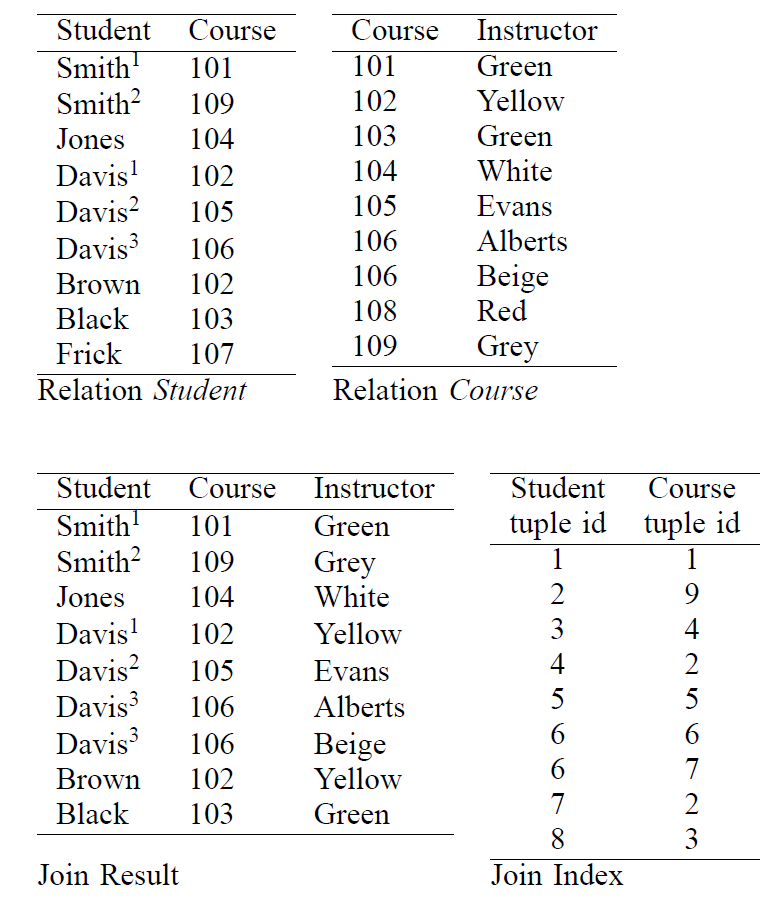
\includegraphics[width=\textwidth,height=0.800\textheight,keepaspectratio]{jive-start.png} 
\footnote{\tiny{Изображение взято из \cite{Li1999}}}
\end{figure}   

\end{frame}

\begin{frame}
\frametitle{Jive Join пример II}

Шаги J1 и J2:

Фрагменты: a) id < 3, b) 3 <= id < 6 и c) 6 <= id.

\begin{figure}[htb]
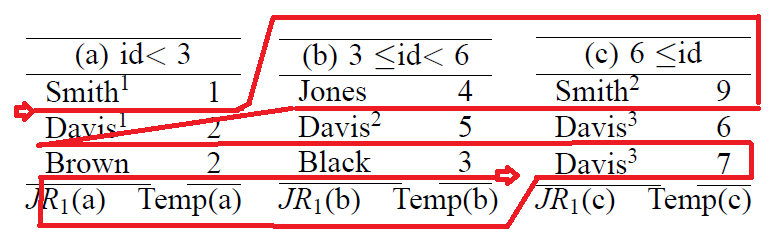
\includegraphics[width=\textwidth,height=0.800\textheight,keepaspectratio]{jive-1.png} 
\footnote{\tiny{Изображение взято из \cite{Li1999}}}
\end{figure}

Слева $JR_1$, справа temporary output file.

\end{frame}

\begin{frame}
\frametitle{Jive join II}

J3 (начало): читаем по отдельности набор \underline{temporary file}
\begin{itemize}
	\setlength\itemsep{1em}
	\item грузим весь фрагмент в память, сортируем в памяти $R_2$ tuple id, по возрастанию, удаляем дубликаты + храним исходную версию во временном файле;
	\item читаем по порядку записи из $R_2$, если совпало -- пишем в $JR_2$;
	\item место определяем по старому порядку, строим над ним хеш, как вариант;
\end{itemize}


\end{frame}


\begin{frame}
\frametitle{Jive Join пример II}

Шаг J3 (начало):

\begin{figure}[htb]
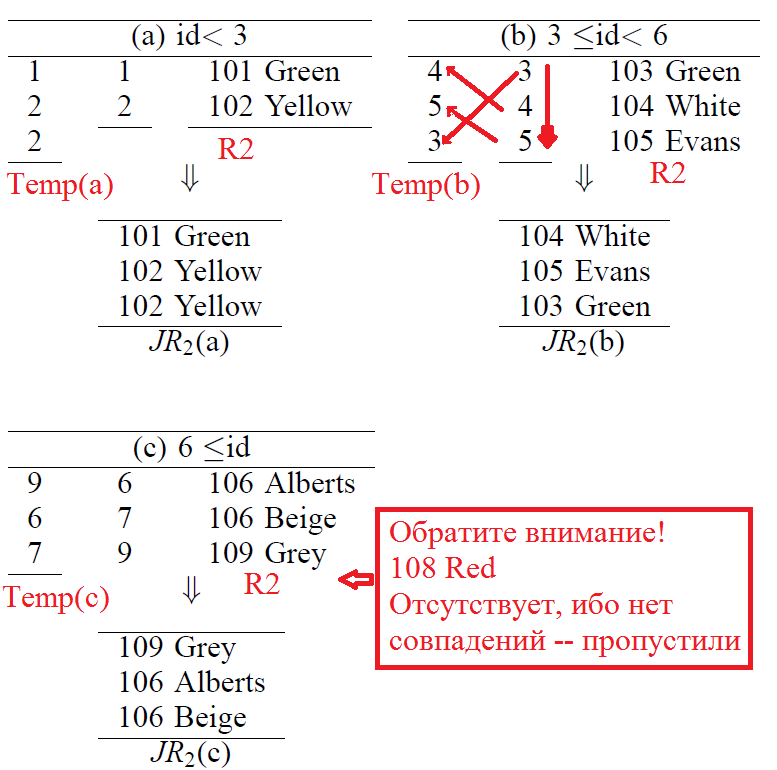
\includegraphics[width=\textwidth,height=0.75\textheight,keepaspectratio]{jive-2.png} 
\footnote{\tiny{Изображение взято из \cite{Li1999}}}
\end{figure}

\end{frame}

\begin{frame}
\frametitle{Jive Join пример III}

Шаг J3 (продолжение): склеиваем $JR_1(x)$ и $JR_2(x)$, последовательно берем каждую пару фрагментов и выполняем ``склейку''.

\begin{figure}[htb]
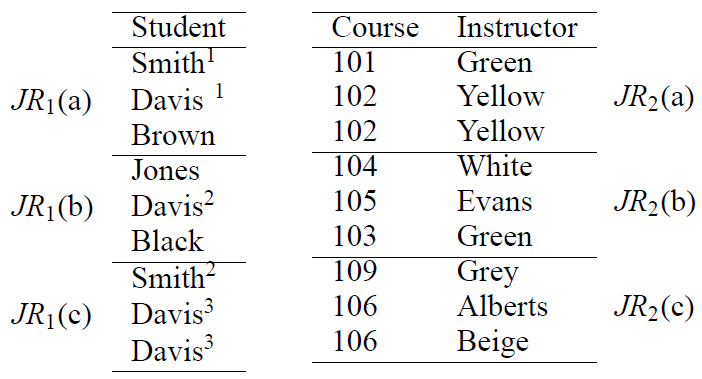
\includegraphics[width=\textwidth,height=0.65\textheight,keepaspectratio]{jive-3.png} 
\footnote{\tiny{Изображение взято из \cite{Li1999}}}
\end{figure}

\end{frame}


\begin{frame}
\frametitle{Jive join: характеристика и итоги}

Плюсы:
\begin{itemize}
  \item Почти весь ввод/вывод последовательный;
  \item Блок читается с диска только если есть запись участвующая в соединении;
  \item $J$ читается единожды;
  \item Временных файлов размером в половину от $J$ сначала пишут, потом читают;
  \item Однопроходен по $R_1$ и $R_2$ (если хватит памяти);
  \item Со skew можно побороться (см. equi-depth, Лекция 4);
\end{itemize}

Минусы:
\begin{itemize}
  \item Ломается pipelining, ждем конца J1 и J2;
  \item Нужен диск на промежуточные результаты~--- $JR_1$ + t. output files; 
  \item Есть ограничения по оперативной памяти на $R_2$ (меньшее отношение), расчеты в статье;
\end{itemize}

\end{frame}

\begin{frame}
\frametitle{Про диск II (latency, iops, throughput)}

\begin{figure}[htb]
	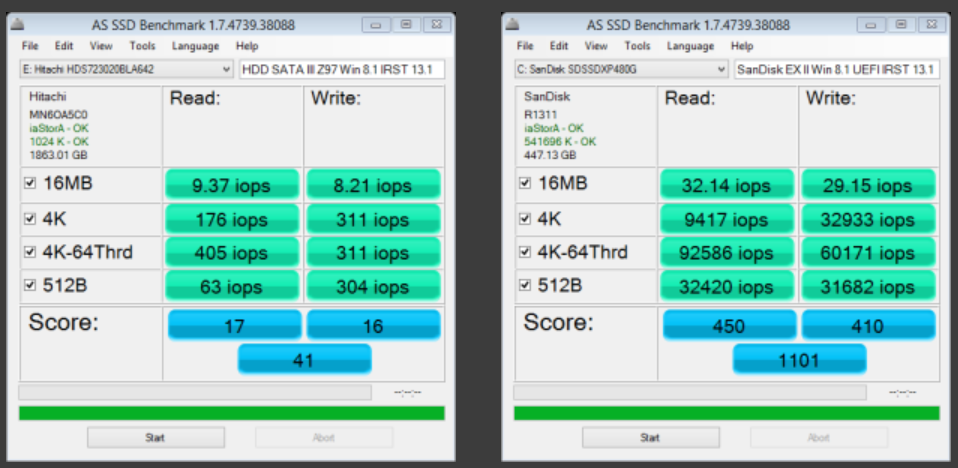
\includegraphics[width=\textwidth,height=0.5\textheight,keepaspectratio]{SSD-vs-HDD-1.png} 
\end{figure}
\vspace{-5.5em}
\begin{figure}[htb]
	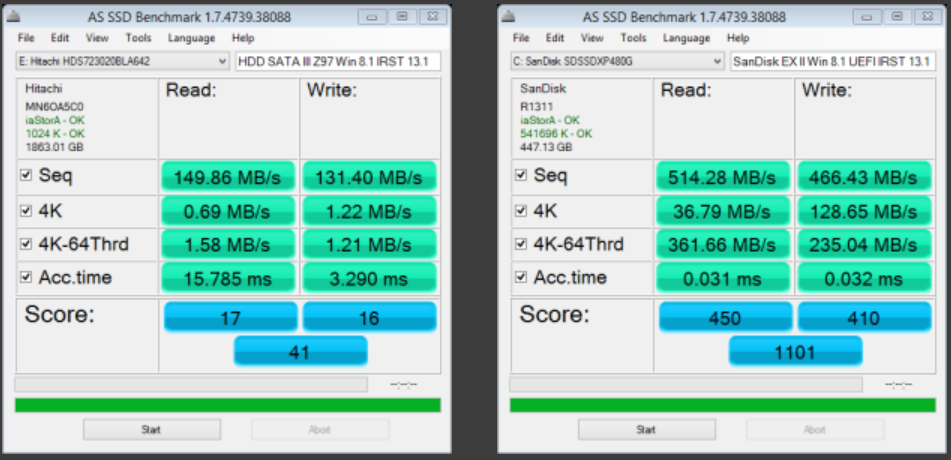
\includegraphics[width=\textwidth,height=0.5\textheight,keepaspectratio]{SSD-vs-HDD-2.png} 
	\footnote{\tiny{Изображения взяты из \url{http://www.thessdreview.com/featured/ssd-throughput-latency-iopsexplained/}}}
\end{figure}

\begin{textblock}{0.5}(0.001, 5)
IOPS
\end{textblock}

\begin{textblock}{0.5}(0.001, 9)
THROUGHPUT	
\end{textblock}

\begin{textblock}{0.5}(5, 1.75)
HDD	
\end{textblock}

\begin{textblock}{0.5}(10, 1.75)
SSD
\end{textblock}

\end{frame}

\begin{frame}
\frametitle{FlashJoin ``на пальцах'' I}

\begin{figure}[htb]
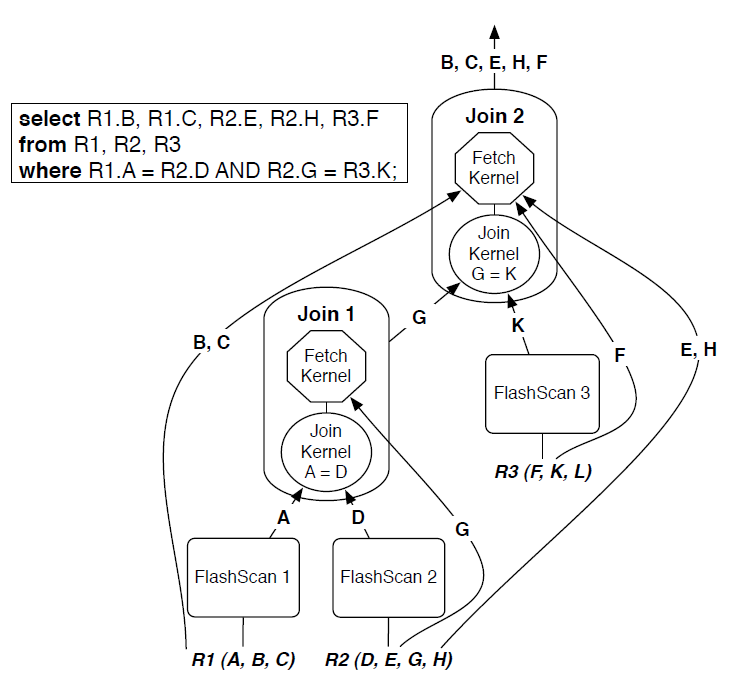
\includegraphics[width=\textwidth,height=0.75\textheight,keepaspectratio]{flashjoin.png} 
\footnote{\tiny{Изображение взято из \cite{Tsirogiannis2009}}}
\end{figure}

\end{frame}


\begin{frame}
\frametitle{FlashJoin ``на пальцах'' II}

Идея: используем быстрые random reads на SSD.

\begin{itemize}
  \item Multi-way equi-join, реализованный как последовательность бинарных;
  \item Каждый бинарный состоит из join kernel и fetch kernel;
  \item Join kernel выдает join index, содержит $(RID, attr_1, attr_2)$;
  \item Fetch kernel по $RID$ считывает нужный атрибут для следующего соединения;
  \item Поздняя материализация результата;
  \item Меньше читаем с диска, меньше ходит между операторами (J)~-- более эффективен по памяти, меньше вероятность многопроходности;
\end{itemize}

\end{frame}

\begin{frame}
\frametitle{Как использовать?}

Проблема: первый случай в Invisible Join III, position lookup идет не последовательно (и пусть отношение больше памяти), производительность страдает от дисковой seek latency.\\~\\

Идея:
\begin{itemize}
  \item Добавить колонку, которая занумерует (1, 2, 3, ...) колонку вычитки из таблицы измерения;
  \item Отсортировать по второй колонке (позициям на поиск);
  \item Сделать соединение, используя последовательное чтение;
  \item Отсортировать по первой колонке и ``подклеить''.
\end{itemize}

Подробный алгоритм смотрите в \cite{Harizopoulos2009}.

\end{frame}

\begin{frame}
\frametitle{Поздняя материализация и соединения, итог}

\begin{itemize}
  \item если применять ``В лоб'' ~--- всё портится, медленнее в 2 раза по сравнению с ранней из-за ``дергания'' диска;
  \item Использовав трюки наподобие Invisible Join, Jive Join, Flash Join, Radix Cluster/Decluster ~--- для некоторых запросов можно добиться что поздняя материализация станет в 2 раза лучше ранней.
\end{itemize}

Это исследования, индустрия же не верит (-ла в 2009, как минимум): используют LM планы только когда неотсортированная колонка вкладывается в память целиком (можем дешево отсортировать).\\~\\

Около 2013 индустрия полностью разочаровалась в LM, кажется что Vertica (наследник C-Store) убрала ее и заменила на SIP (sideways information passing). Однако, диски стали в этот период сильно лучше и поэтому на мой взгляд будущее у этой идеи есть.

\end{frame}


\begin{frame}
\frametitle{Сравнение row-store и column-store\footnote{есть на русском \url{citforum.ru/database/articles/column\_vs\_row\_store/}}}

Эмуляция колоночной СУБД в System-X \cite{Abadi2008}:
\begin{itemize}
  \setlength\itemsep{1em}
  \item VP: Полное вертикальное фрагментирование (ключ, атрибут);
  \begin{itemize}
    \item Соединять с помощью HJ, пытались и кластеризованный индекс~--- хуже.
  \end{itemize}
  \item AI: Index-only планы (каждый атрибут проиндексирован), так чтобы не читать таблицы вообще;
  \begin{itemize}
    \item Дополнительный некластеризованный индекс.
  \end{itemize}
  \item MV: Материализованное представление для каждого запроса, только нужные атрибуты, без prejoined tables.
\end{itemize}

Против:
\begin{itemize}
  \setlength\itemsep{1em}
  \item T: Дефолтные планы, которые могут использовать битмап индексы и блум фильтры, если сочтет нужным;
  \item T(B): Дефолтные планы с битмап индексами.
\end{itemize}


\end{frame}

\begin{frame}
\frametitle{Сравнение}

\begin{figure}[htb]
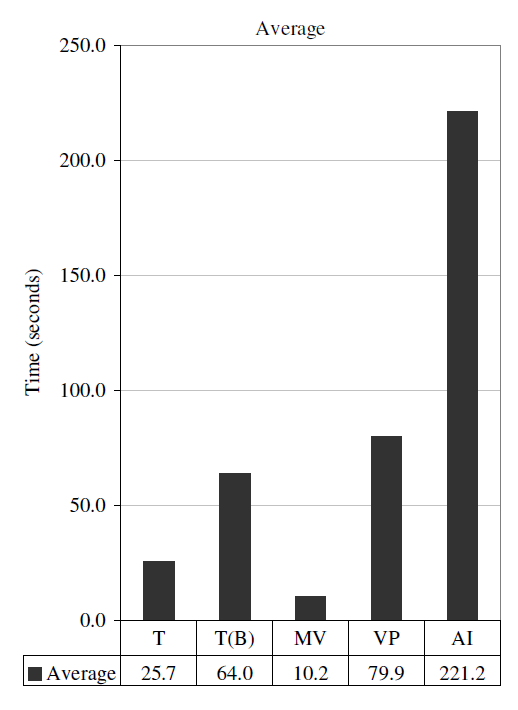
\includegraphics[width=\textwidth,height=0.75\textheight,keepaspectratio]{comp-1.png} 
\footnote{\tiny{Изображение взято из \cite{Harizopoulos2009}}}
\end{figure}

Взяли query 2.1 из Star Schema Benchmark (в C-Store выполнялся 5.7с).

\end{frame}

\begin{frame}
\frametitle{Какие особенности CS дают большее преимущество?}

Особенности \cite{Abadi2008}:
\begin{itemize}
  \setlength\itemsep{1em}
  \item Одна запись vs несколько записей;
  \item Invisible Join;
  \item Сжатие;
  \item Поздняя материализация;
\end{itemize}


Легенда (конфигурация C-Store):
\begin{itemize}
  \item T=tuple-at-a-time processing, t=block processing;
  \item I=invisible join enabled, i=disabled;
  \item C=compression enabled, c=disabled;
  \item L=late materialization enabled, l=disabled. 
\end{itemize}

\end{frame}


\begin{frame}
\frametitle{Какие особенности CS дают большее преимущество: сравнение}

\begin{figure}[htb]
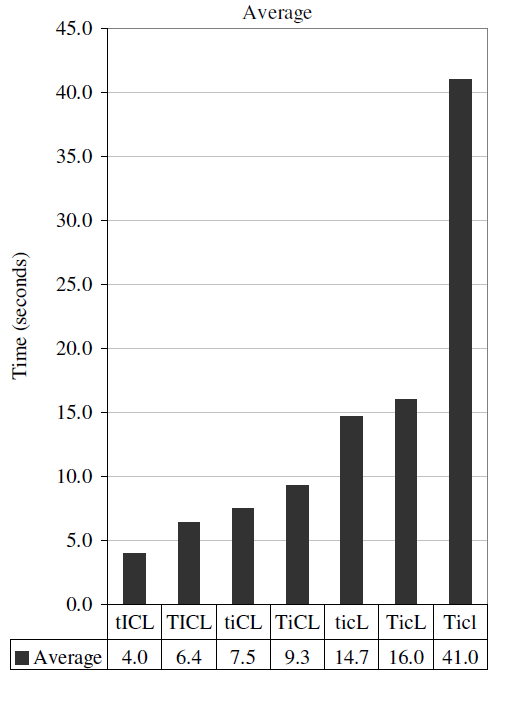
\includegraphics[width=\textwidth,height=0.75\textheight,keepaspectratio]{comp-2.png} 
\footnote{\tiny{Изображение взято из \cite{Harizopoulos2009}}}
\end{figure}

\end{frame}


\begin{frame}
\frametitle{Изображения}

Большинство изображений взяты из оригиналов статей или прямо из слайдов \cite{Harizopoulos2009}.

\end{frame}


\begin{frame}[allowframebreaks]
\frametitle{Ссылки}
\footnotesize{
\begin{thebibliography}{99}

\bibitem[Tsirogiannis et al., 2009] {Tsirogiannis2009}  Dimitris Tsirogiannis, Stavros Harizopoulos, Mehul A. Shah, Janet L. Wiener, and Goetz Graefe. 2009. Query processing techniques for solid state drives. In Proceedings of the 2009 ACM SIGMOD International Conference on Management of data (SIGMOD '09), Carsten Binnig and Benoit Dageville (Eds.). ACM, New York, NY, USA, 59-72. DOI=http://dx.doi.org/10.1145/1559845.1559854 

\bibitem[Li and Ross, 1999] {Li1999} Zhe Li and Kenneth A. Ross. 1999. Fast joins using join indices. The VLDB Journal 8, 1 (April 1999), 1--24. DOI=http://dx.doi.org/10.1007/s007780050071 

\bibitem[Star Schema Benchmark Specification, 2009] {SSB} Star Schema Benchmark. Revision 3, June 5, 2009 Pat O'Neil, Betty O'Neil, Xuedong Chen

\bibitem[Abadi et al., 2008] {Abadi2008} Daniel J. Abadi, Samuel R. Madden, and Nabil Hachem. 2008. Column-stores vs. row-stores: how different are they really?. In Proceedings of the 2008 ACM SIGMOD international conference on Management of data (SIGMOD '08). ACM, New York, NY, USA, 967-980. DOI=http://dx.doi.org/10.1145/1376616.1376712 

\bibitem[TPC-H Specification, 2011] {TPC-H} TPC BENCHMARK(TM) H (Decision Support) Standard Specification Revision 2.14.2

\bibitem[Abadi et al., 2012] {Abadi2013} Daniel Abadi, Peter Boncz, Stavros Harizopoulos. The Design and Implementation of Modern Column-Oriented Database Systems. Foundations and Trends(R) in Databases Vol. 5, No. 3 (2012) 197--280

\bibitem[Harizopoulos et al., 2009] {Harizopoulos2009} Stavros Harizopoulos, Daniel Abadi, Peter Boncz. Column-Oriented Database Systems. VLDB 2009 Tutorial (slides).

% \bibitem[Чернышев, 2013] {Chernishev2013}	Г. А. Чернышев, <<Организация физического уровня колоночных СУБД>>, Тр. СПИИРАН, 30 (2013), 204--222

% \bibitem[Кузнецов, 2010] {Kuznetsov2010}	 Кузнецов С.Д., <<Год эпохи перемен в технологии баз данных>>, Труды Института системного программирования РАН, 19 (2010), 9--34

%\bibitem[Elnikety, 2009] {Elnikety2009} Distributed DBMS. Sameh Elnikety. Encyclopedia of Database Systems. Ling Liu and M. Tamer {\"O}zsu (eds), p. 896--899. Springer US, 2009. \url{http://dx.doi.org/10.1007/978-0-387-39940-9\_654}

%\bibitem[Kian-Lee Tan, 2009] {Kian-Lee2009} Distributed Database Systems. Kian-Lee Tan. Encyclopedia of Database Systems. Ling Liu and M. Tamer {\"O}zsu (eds), p. 894--896. Springer US, 2009. \url{http://dx.doi.org/10.1007/978-0-387-39940-9_701}

%\bibitem[{\"O}zsu and Valduriez, 2009] {Ozsu2011} {\"O}zsu M.T. and Valduriez P. Principles of Distributed Database Systems, 3rd ed. Prentice-Hall, 2011.

%\bibitem[Kossmann, 2000] {Kossmann2000} Donald Kossmann. 2000. The state of the art in distributed query processing. ACM Comput. Surv. 32, 4 (December 2000), 422--469. DOI=http://dx.doi.org/10.1145/371578.371598 


%\bibitem[Ioannidis, 2003] {Ioannidis2003}  Yannis Ioannidis. 2003. The history of histograms (abridged). In Proceedings of the 29th international conference on Very large data bases - Volume 29 (VLDB '03), Johann Christoph Freytag, Peter C. Lockemann, Serge Abiteboul, Michael J. Carey, Patricia G. Selinger, and Andreas Heuer (Eds.), Vol. 29. VLDB Endowment 19--30. 

%\bibitem[Ioannidis and Poosala, 1995] {Ioannidis1995} Y. Ioannidis and V. Poosala. Histogram Based Solutions to Diverse Database Estimation Problems, IEEE Data Engineering, Vol. 18, No. 3, pp. 10--18, September 1995.

%\bibitem[Poosala et al., 1996] {Poosala1996} Viswanath Poosala, Peter J. Haas, Yannis E. Ioannidis, and Eugene J. Shekita. 1996. Improved histograms for selectivity estimation of range predicates. In Proceedings of the 1996 ACM SIGMOD international conference on Management of data (SIGMOD '96), Jennifer Widom (Ed.). ACM, New York, NY, USA, 294--305. DOI=http://dx.doi.org/10.1145/233269.233342 


%\bibitem[Kooi, 1980] {Kooi1980} Robert Philip Kooi. The Optimization of Queries in Relational Databases. PhD Thesis, Case Western Reserve University (1980).

%\bibitem[Piatetsky-Shapiro and Connel, 1984] {Piatetsky-Shapiro1984} Gregory Piatetsky-Shapiro and Charles Connell. 1984. Accurate estimation of the number of tuples satisfying a condition. In Proceedings of the 1984 ACM SIGMOD international conference on Management of data (SIGMOD '84). ACM, New York, NY, USA, 256--276. DOI=http://dx.doi.org/10.1145/602259.602294 


%\bibitem[Garcia-Molina et al., 2004] {Ulman2004} Гектор Гарсиа-Молина, Джеффри Д. Ульман, Дженнифер Уидом. Системы баз данных. Полный курс.  ISBN 5-8459-0384-Х; 2004 г. 

%\bibitem[Hellerstein et al., 2007] {Hellerstein2007} Joseph M. Hellerstein, Michael Stonebraker, and James Hamilton. Architecture of a Database System. Found. Trends databases 1, 2 (February 2007), 141--259. 

%\bibitem[Neumann, 2009] {Neumann2009} Thomas Neumann. Query Optimization (in Relational Databases). Encyclopedia of Database Systems. Springer US, 2009. 2273--2278.\url{http://dx.doi.org/10.1007/978-0-387-39940-9_293}

%\bibitem[Selinger et al., 1979] {Selinger1979} Selinger P.G., Astrahan M.M., Chamberlin D.D., Lorie R.A., and Price T.G. Access path selection in a relational database management System. In Proc. ACM SIGMOD Int. Conf. on Management of Data, 1979, pp. 23--34.

%\bibitem[Haas et al., 1989] {Haas1989} Haas L.M., Freytag J.C., Lohman G.M., and Pirahesh H. Extensible query processing in starburst. In Proc. ACM SIGMOD Int. Conf. on Management of Data, 1989, pp. 377--388.

%\bibitem[Graefe, 1995] {Graefe1995} Graefe G. The cascades framework for query optimization. Q. Bull. IEEE TC on Data Engineering, 18(3):19--29, 1995.

%\bibitem[Graefe and McKenna, 1993] {Graefe1993} Graefe G. and McKenna W.J. The volcano optimizer generator: Extensibility and efficient search. In Proc. 9th Int. Conf. on Data Engineering, 1993, pp. 209--218.

%\bibitem[Chaudhuri, 1998] {Chaudhuri1998} Chaudhuri S. An overview of query optimization in relational systems. In Proc. 17th ACM SIGACT-SIGMOD-SIGART Symp. Principles of Database Systems, 1998, pp. 34--43.

%\bibitem[Ioannidis, 1996] {Ioannidis1996} Ioannidis Y. Query optimization. In Handbook of Computer Science, A.B. Tucker (ed.). CRC Press, 1996.

%\bibitem[Jarke and Koch, 1984] {Chaudhuri1984} Jarke M. and Koch J. Query optimization in database systems. ACM Comput. Surv., 16(2):111–152, 1984.

%\bibitem[Ioannidis, 1996] {Ioannidis1996} Yannis E. Ioannidis. 1996. Query optimization. ACM Comput. Surv. 28, 1 (March 1996), 121--123. DOI=http://dx.doi.org/10.1145/234313.234367 

%\bibitem[Graefe, 1996] {Graefe1996} Goetz Graefe. 1996. Iterators, schedulers, and distributed-memory parallelism. Softw. Pract. Exper. 26, 4 (April 1996), 427--452. DOI=http://dx.doi.org/10.1002/(SICI)1097-024X(199604)26:4<427::AID-SPE20>3.3.CO;2-8 

%\bibitem[Taniar et al., 2008] {Taniar2008} David Taniar, Clement H. C. Leung, Wenny Rahayu, and Sushant Goel. 2008. High Performance Parallel Database Processing and Grid Databases. Wiley Publishing. 

%\bibitem[Ramakrishnan and Gehrke, 2000] {Ramakrishnan2000}  Raghu Ramakrishnan and Johannes Gehrke. 2000. Database Management Systems (2nd ed.). Osborne/McGraw-Hill, Berkeley, CA, USA. 

\end{thebibliography}
}
\end{frame}


\end{document} 